\documentclass[a4paper,10pt]{article}
\usepackage[utf8]{inputenc}

\usepackage{listings}
\usepackage{color}
\usepackage{graphicx}
\usepackage{float}
\definecolor{codegreen}{rgb}{0,0.6,0}
\definecolor{codegray}{rgb}{0.5,0.5,0.5}
\definecolor{codepurple}{rgb}{0.58,0,0.82}
\definecolor{backcolour}{rgb}{0.95,0.95,0.92}
 
\lstdefinestyle{mystyle}{
    backgroundcolor=\color{backcolour},   
    commentstyle=\color{codegreen},
    keywordstyle=\color{magenta},
    numberstyle=\tiny\color{codegray},
    stringstyle=\color{codepurple},
    basicstyle=\footnotesize,
    breakatwhitespace=false,         
    breaklines=true,                 
    captionpos=b,                    
    keepspaces=true,                 
    numbers=left,                    
    numbersep=5pt,                  
    showspaces=false,                
    showstringspaces=false,
    showtabs=false,                  
    tabsize=2
}
\lstset{style=mystyle}

\title{Orienté Objet \\ Mini Projet - Batlleship}
\author{Arthur Deschamps \& Théo Giovanna }
\date{May 2017}

\begin{document}

\maketitle

\section{Les diagrammes}

\subsection{Diagrammes de classe}

\begin{figure}[H]
    \center
    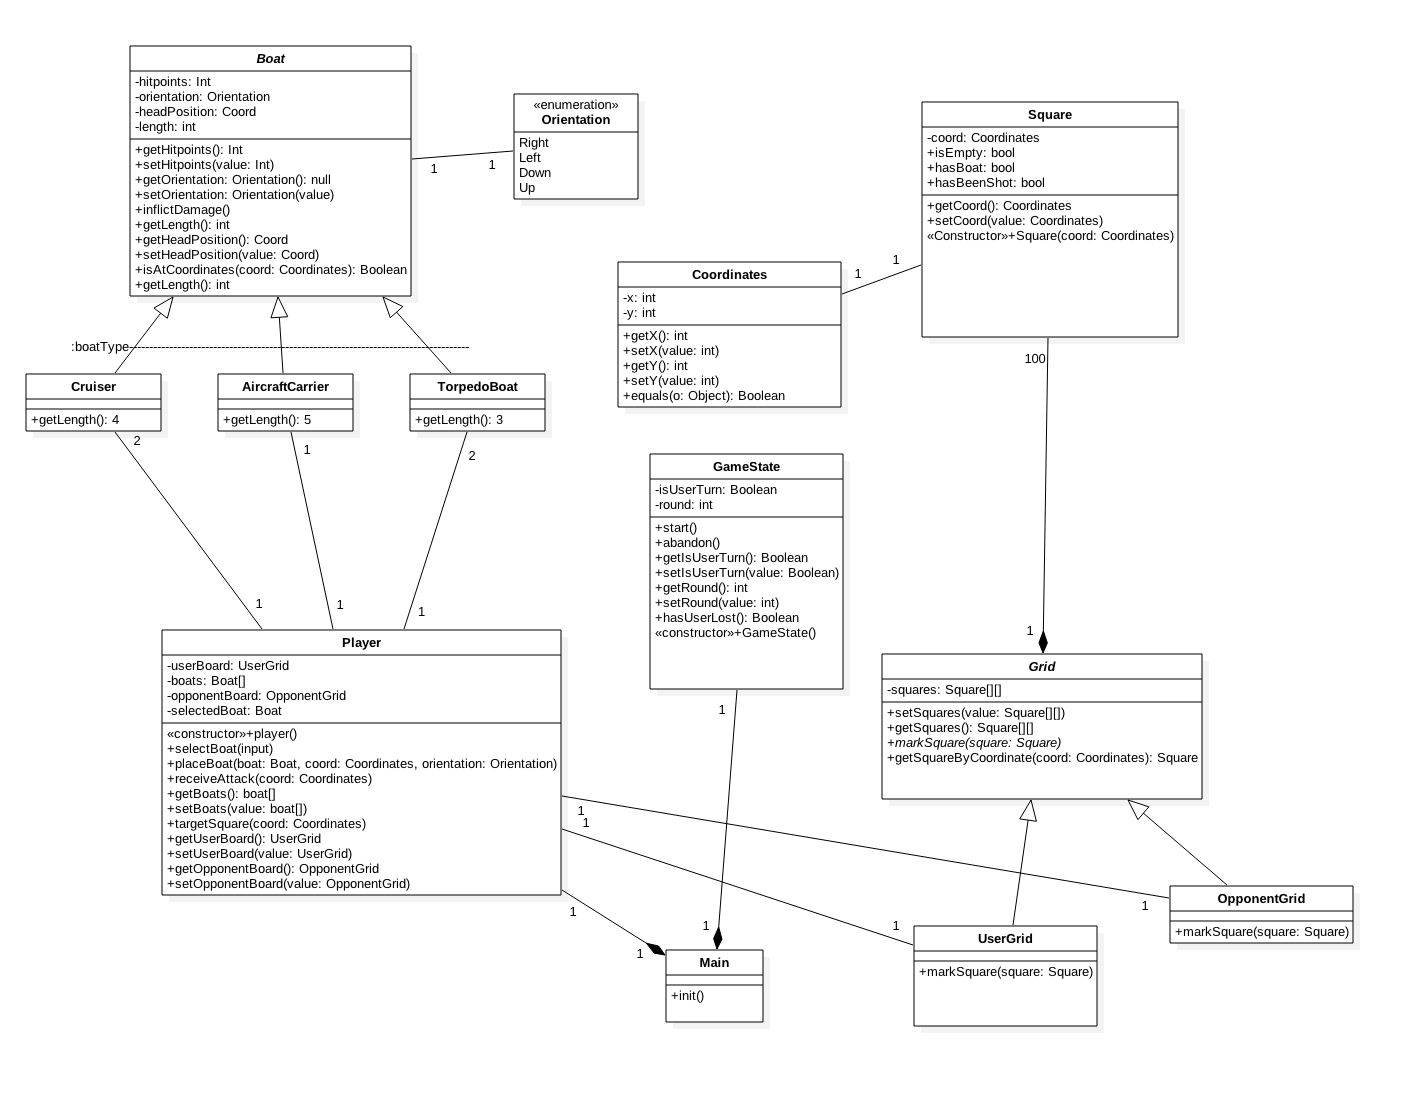
\includegraphics[scale=0.50]{images/mainClass}
    \caption{Méthodes principales}
    \label{fig:my_label}
\end{figure}

\begin{figure}[H]
    \center
    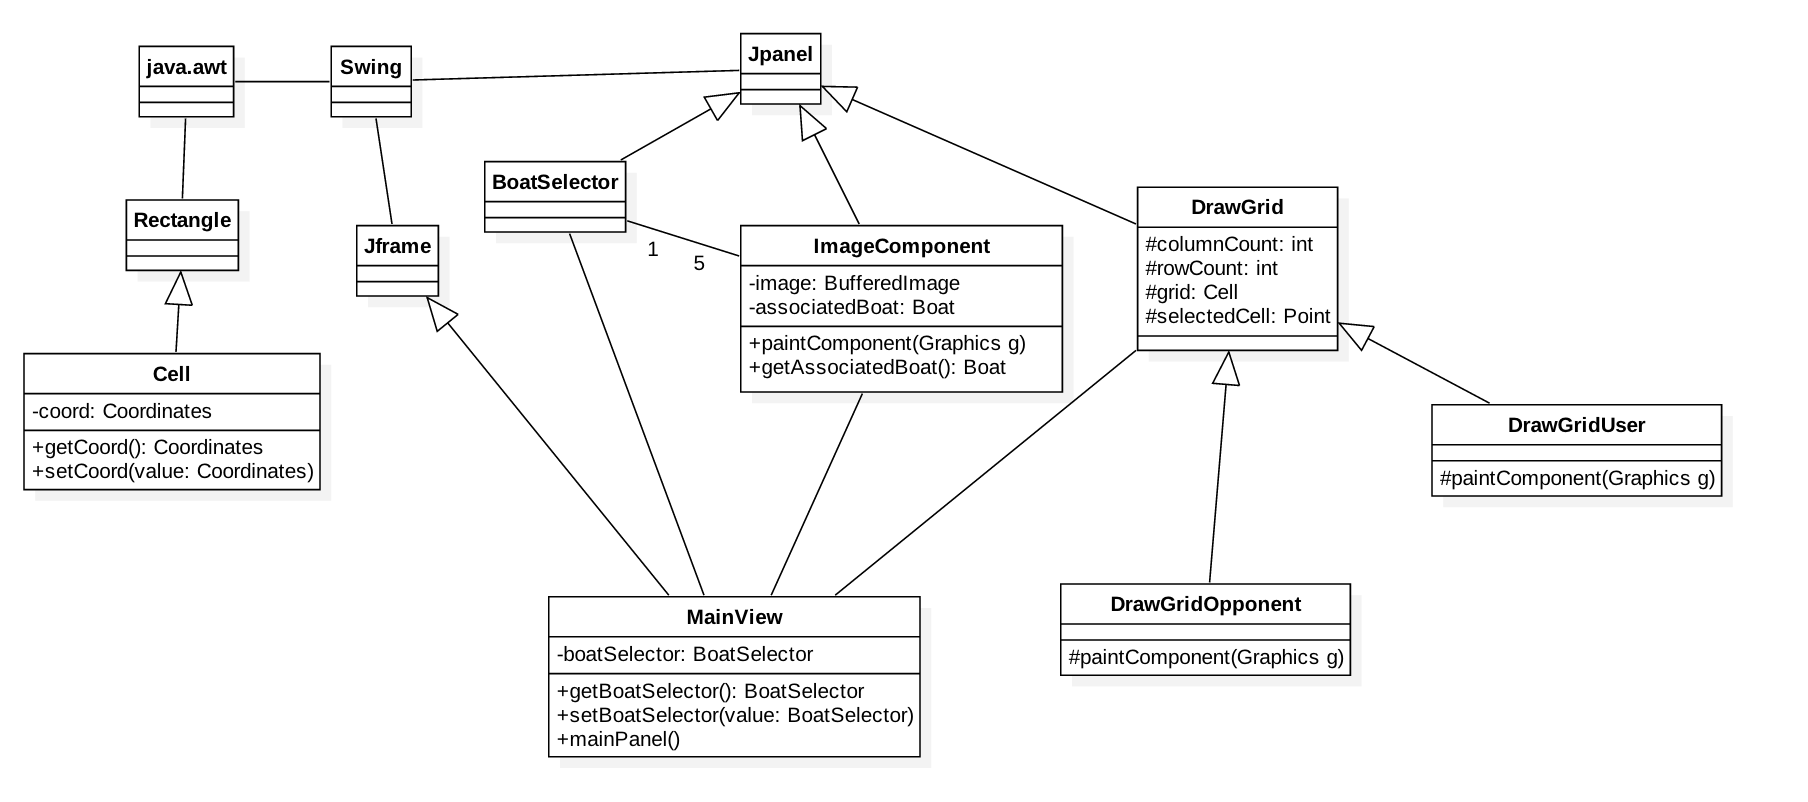
\includegraphics[scale=0.45]{images/guiClass}
    \caption{Interface graphique}
    \label{fig:my_label}
\end{figure}

\subsection{Diagramme de séquence}

\begin{figure}[H]
    \center
    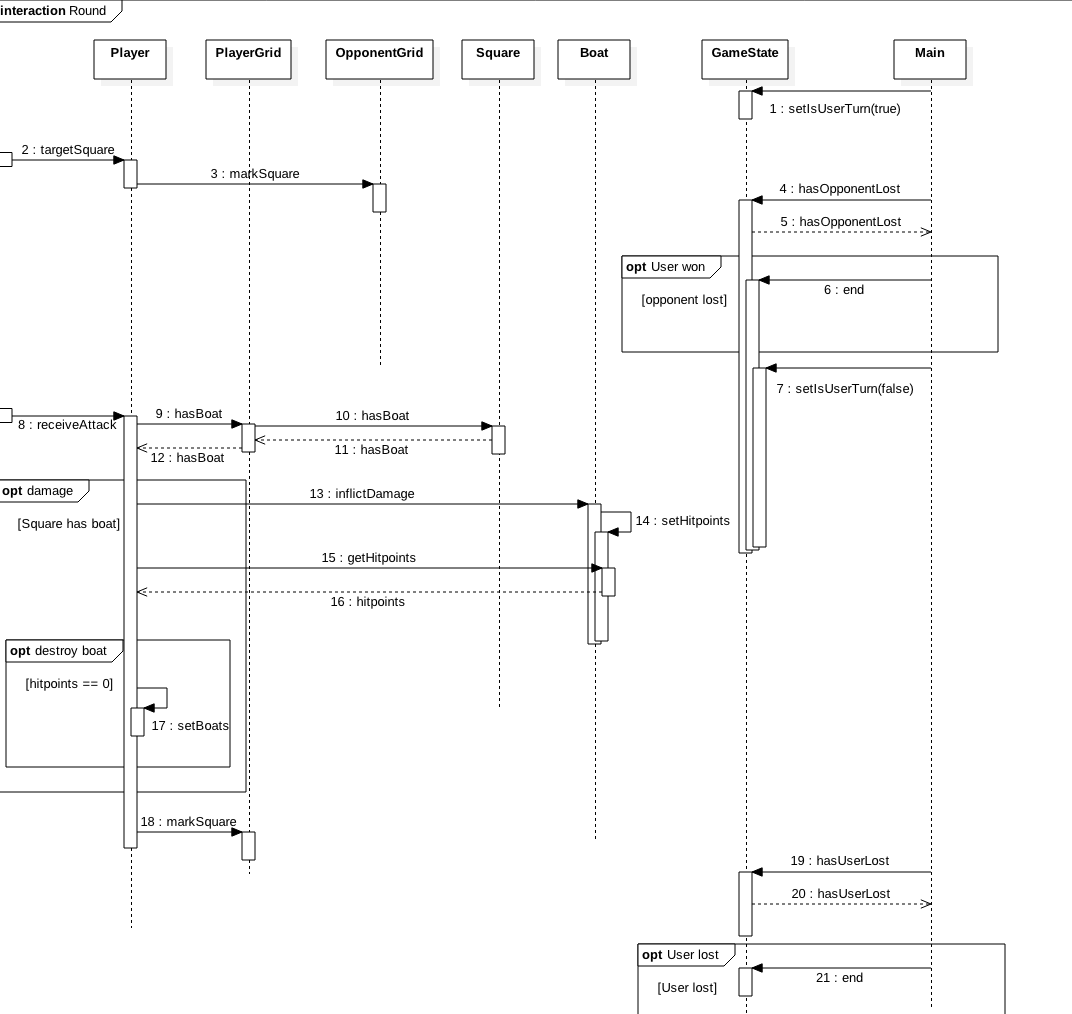
\includegraphics[scale=0.65]{images/sequence}
    \caption{Détail d'un tour d'un joueur}
    \label{fig:my_label}
\end{figure}

\subsection{Diagramme d'états}

\begin{figure}[H]
    \center
    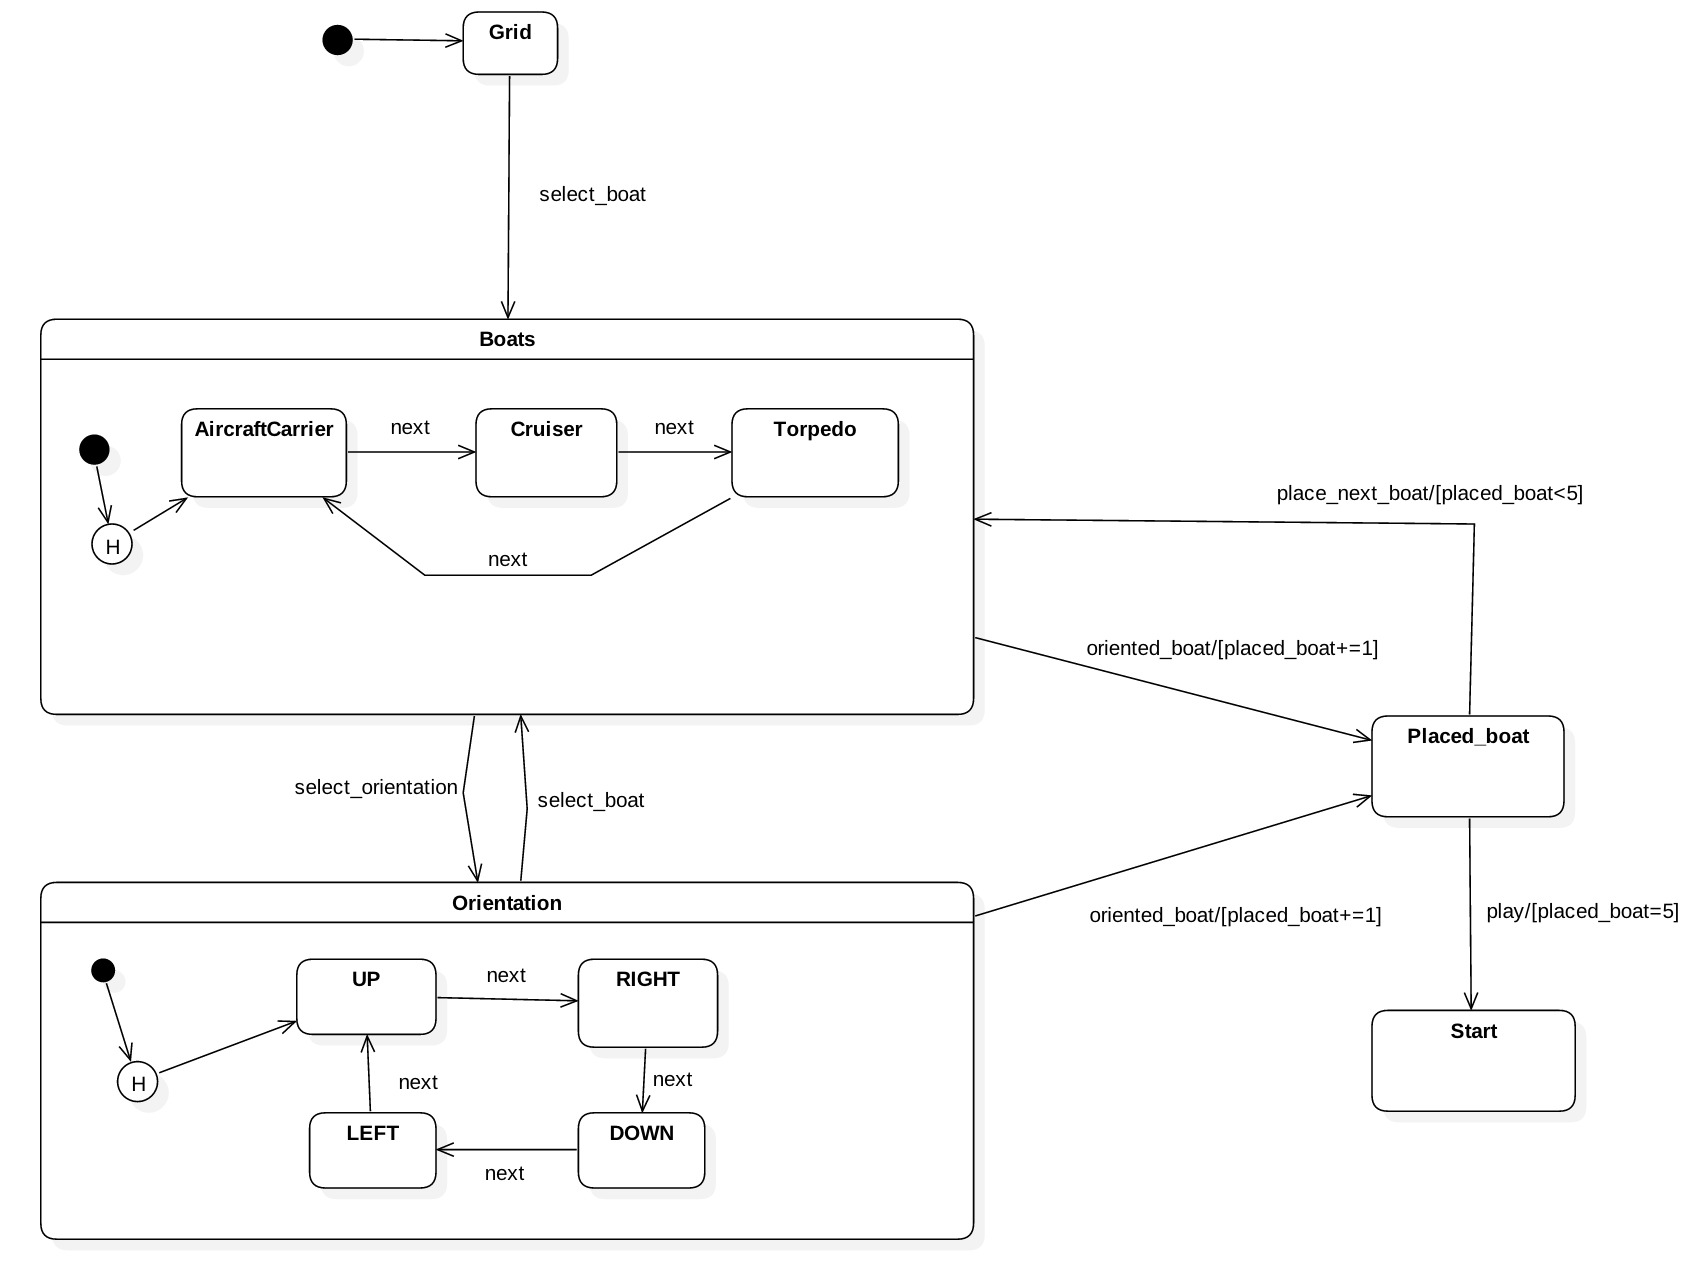
\includegraphics[scale=0.45]{images/action}
    \caption{Sélection et placement d'un bateau}
    \label{fig:my_label}
\end{figure}

\section{Démarrage du jeu}

\subsection{Lancement}

\begin{figure}[H]
    \center
    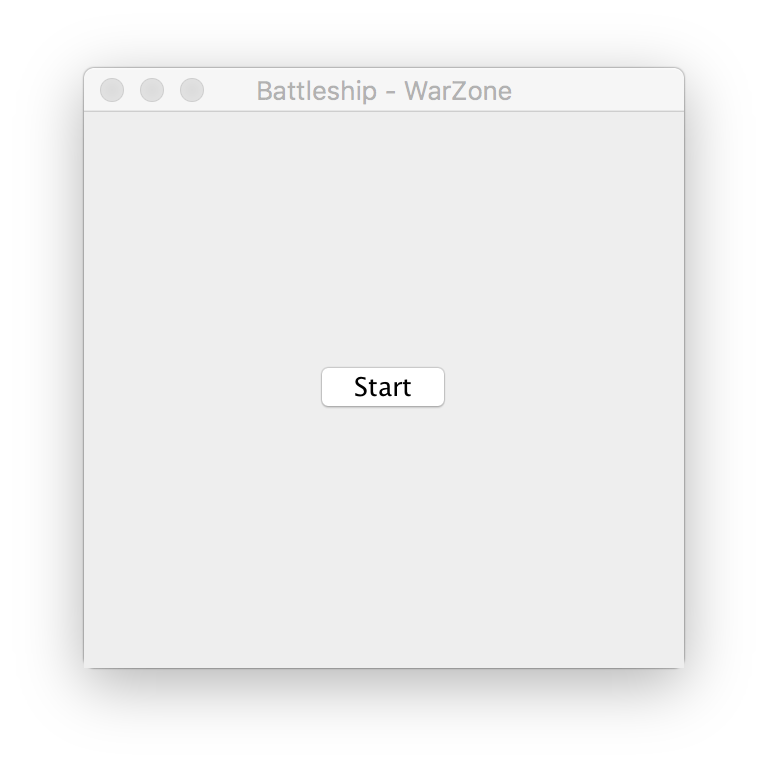
\includegraphics[scale=0.35]{images/start}
    \caption{Lancement du programme}
    \label{fig:my_label}
\end{figure}

\subsection{Acceuil}

\begin{figure}[H]
    \center
    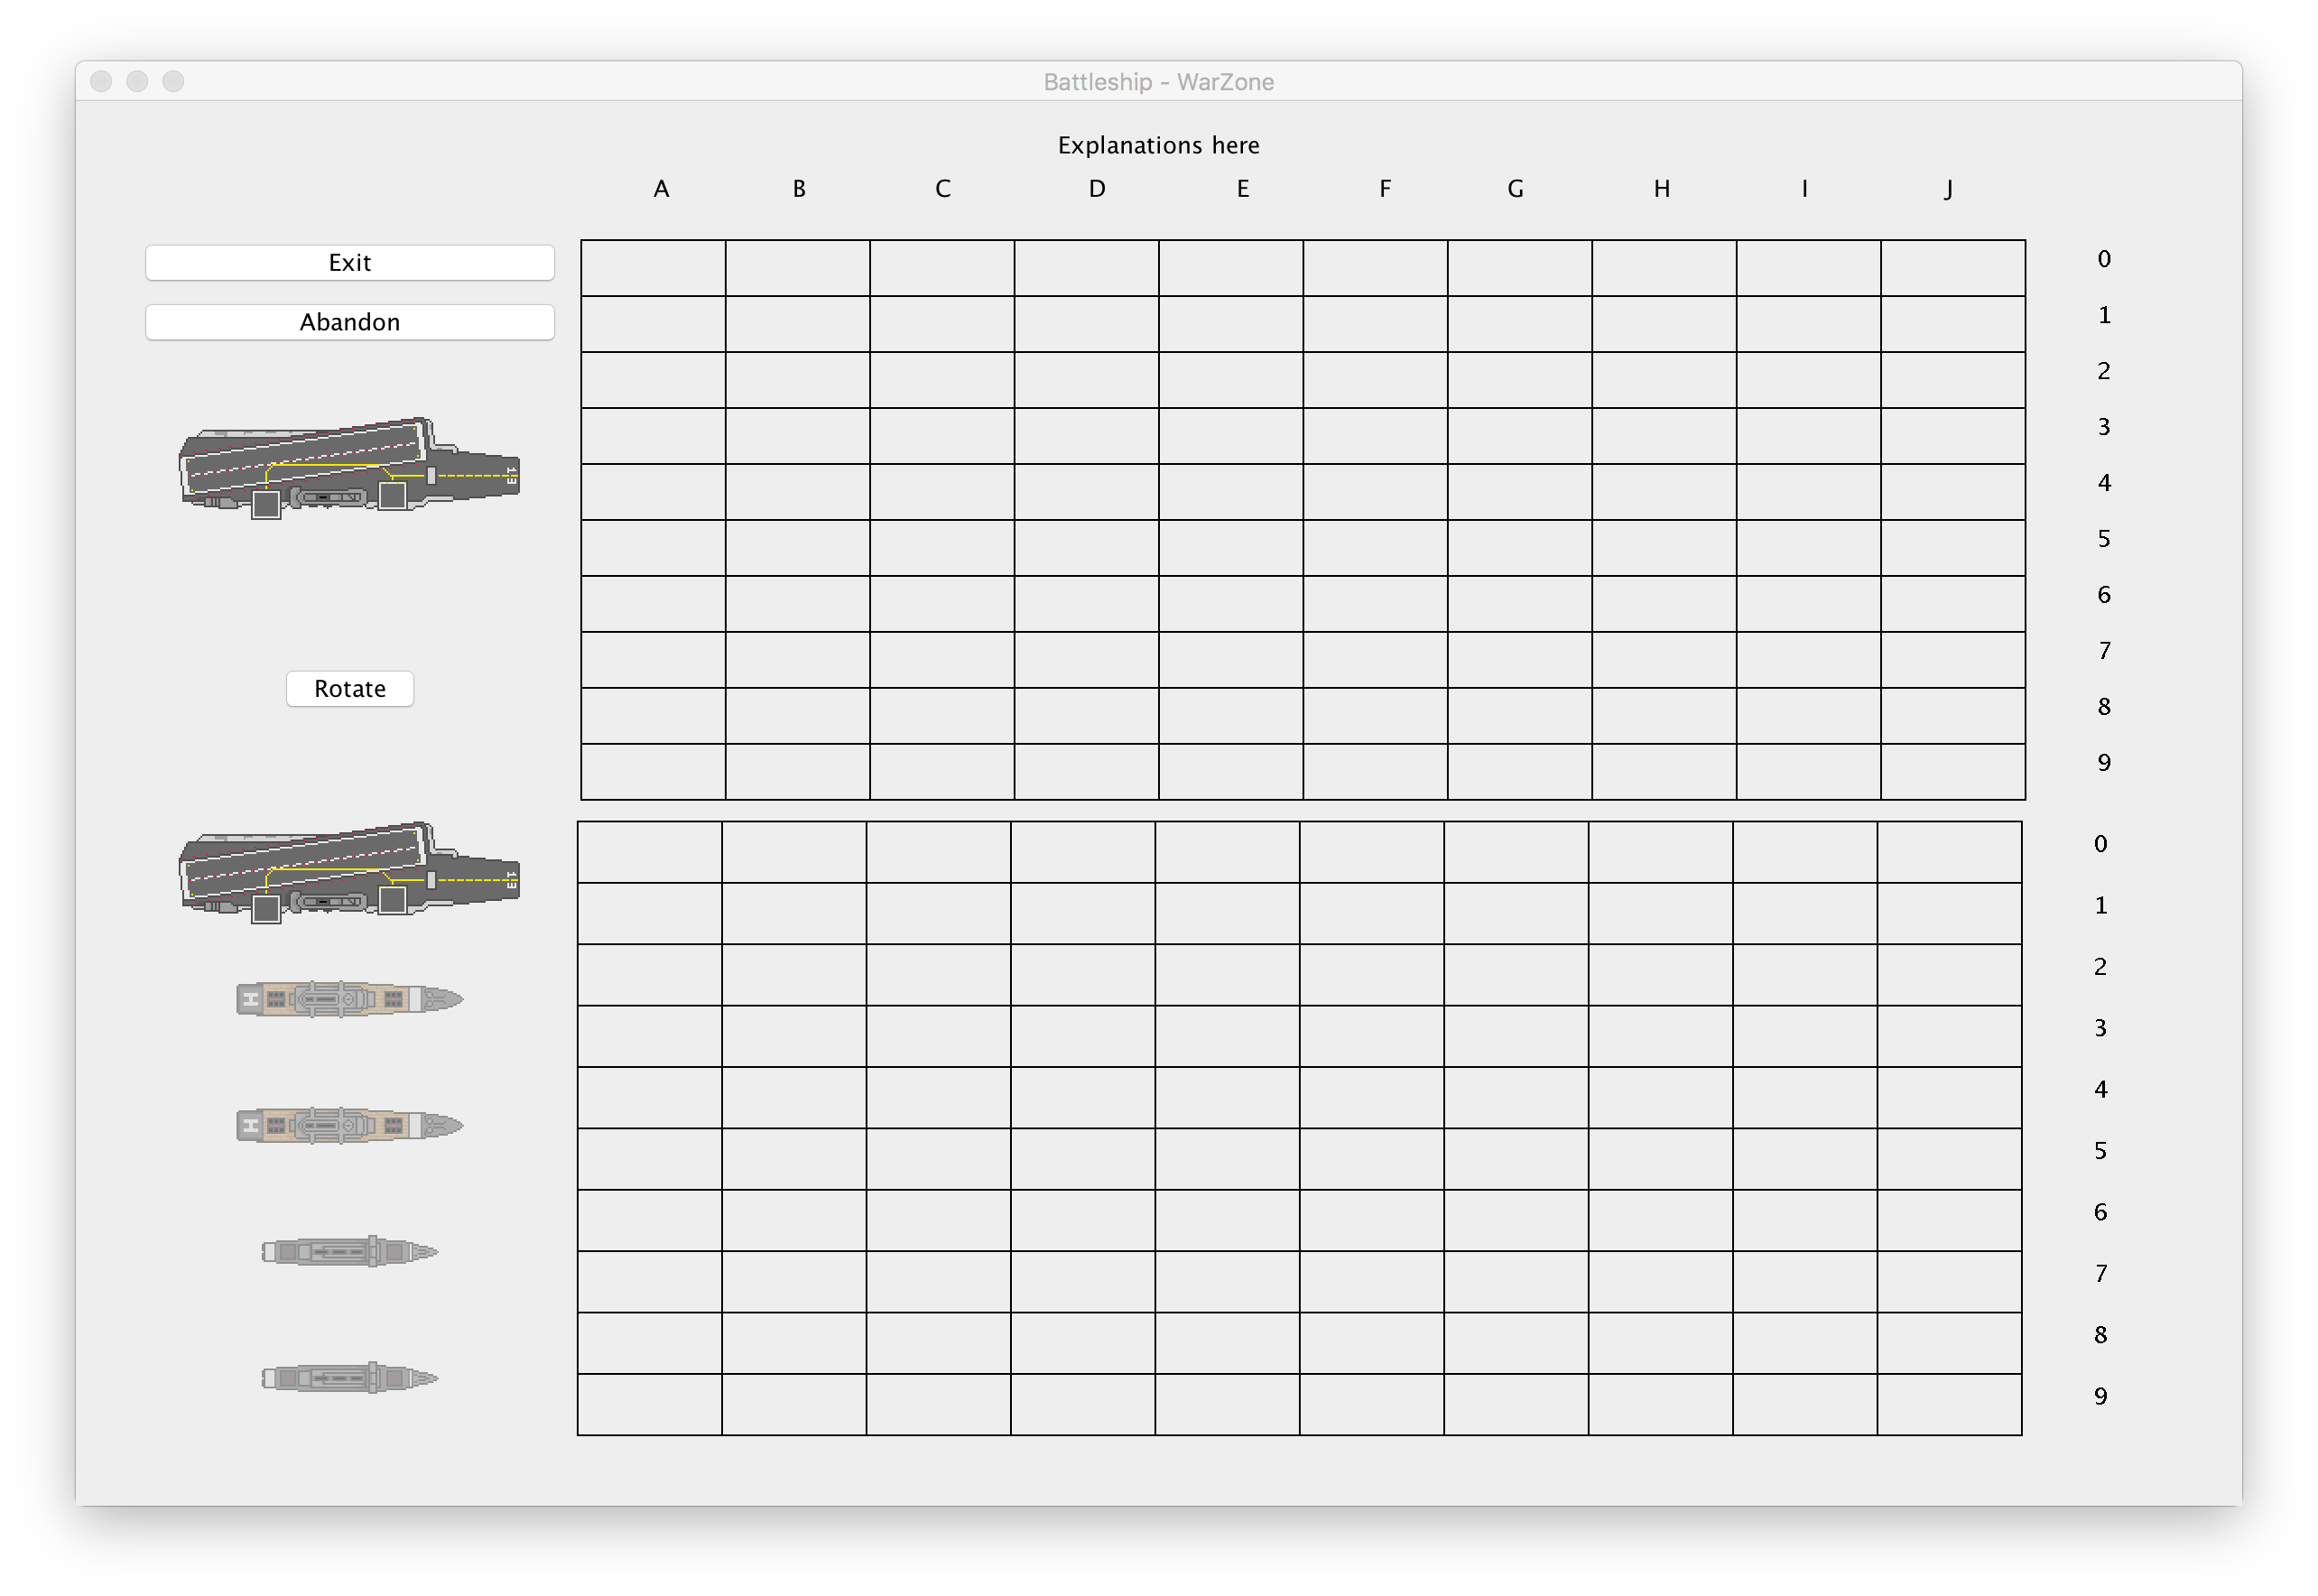
\includegraphics[scale=0.35]{images/acceuil}
    \caption{Lancement du programme}
    \label{fig:my_label}
\end{figure}

\subsection{Grille du joueur adverse}

\begin{figure}[H]
    \center
    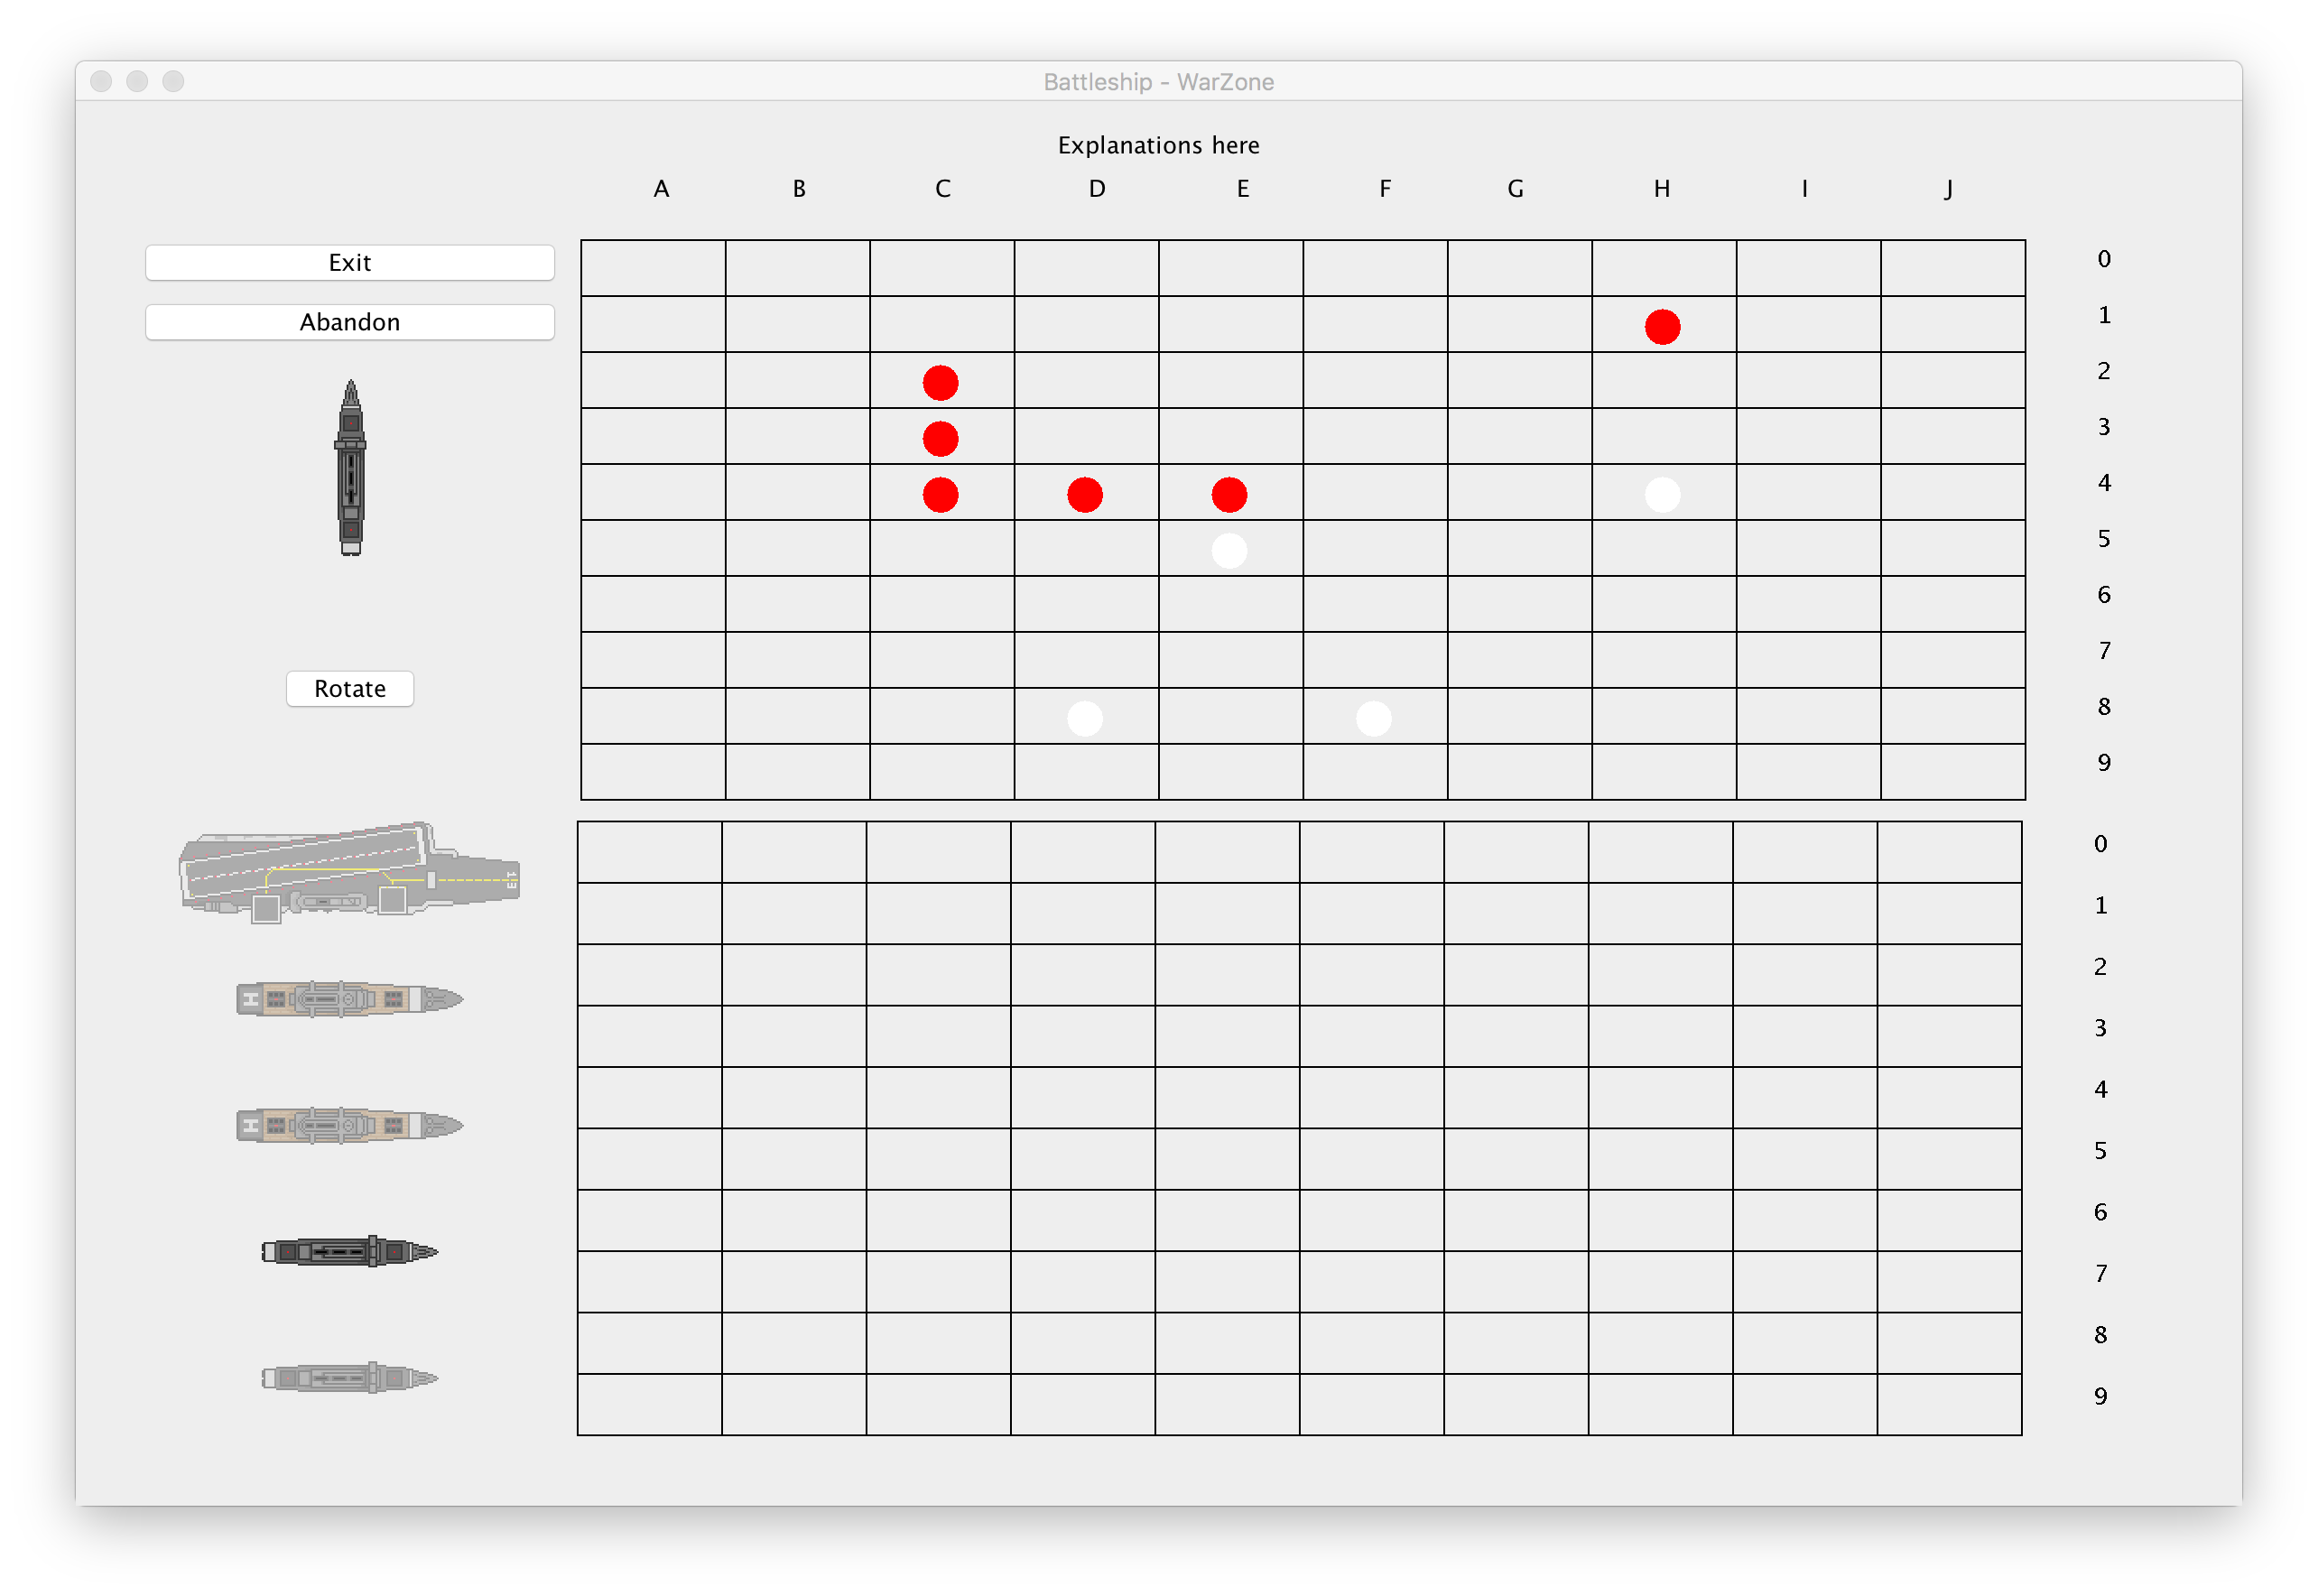
\includegraphics[scale=0.35]{images/encours}
    \caption{Lancement du programme}
    \label{fig:my_label}
\end{figure}

Lorsque l'on clique sur une des cases de la grille opponent, un pop-up s'affiche et nous demande si on a touché un de ses bateaux ou non. Le cas échéant, on affiche un cercle rouge, sinon un blanc.

\subsection{Grille personelle}

Nous avons la possibilité de choisir le bateau désiré ainsi que son orientation pour ensuite le placer sur la grille (ronds bleus)
A tout moment nous pouvons quitter ou abandonner la partie en cours.
\noindent Rond blanc = pas touché, rond rouge = touché.

\noindent Lorsque que tous les ronds bleus sont rouges, alors un message de défaite s'affiche.

\begin{figure}[H]
    \center
    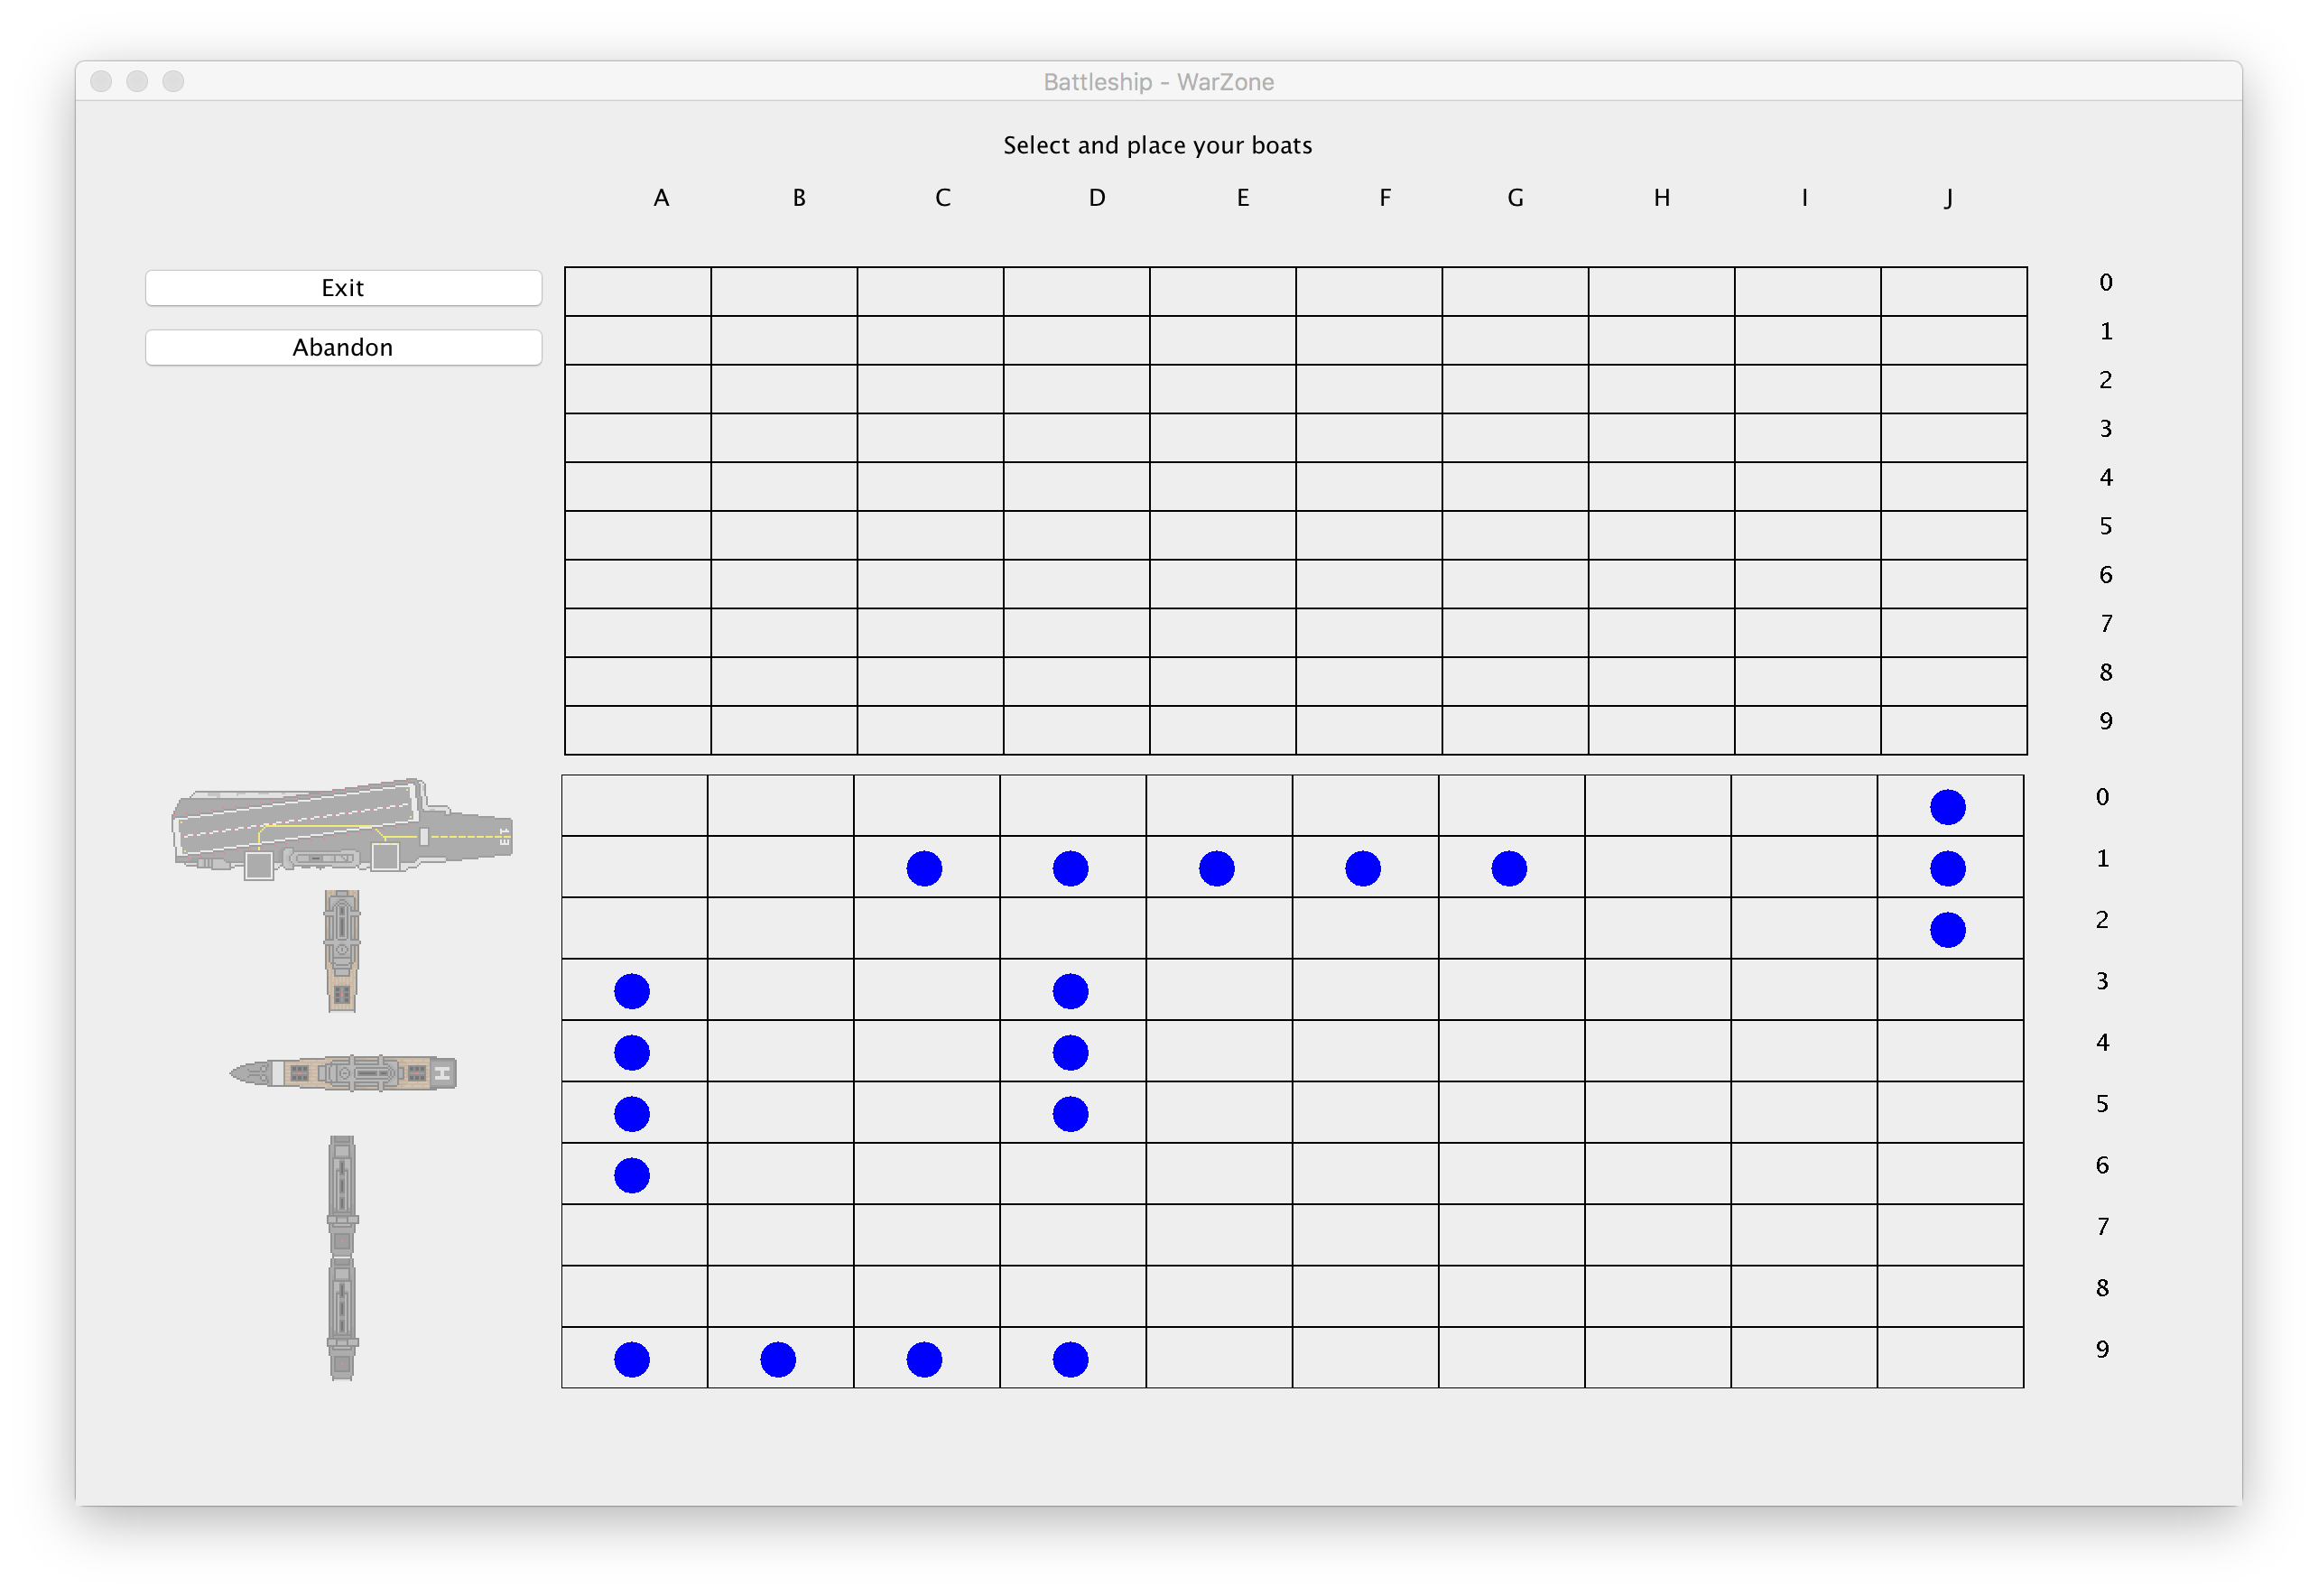
\includegraphics[scale=0.35]{images/placeboat}
    \caption{On place les bateaux}
    \label{fig:my_label}
\end{figure}

\begin{figure}[H]
    \center
    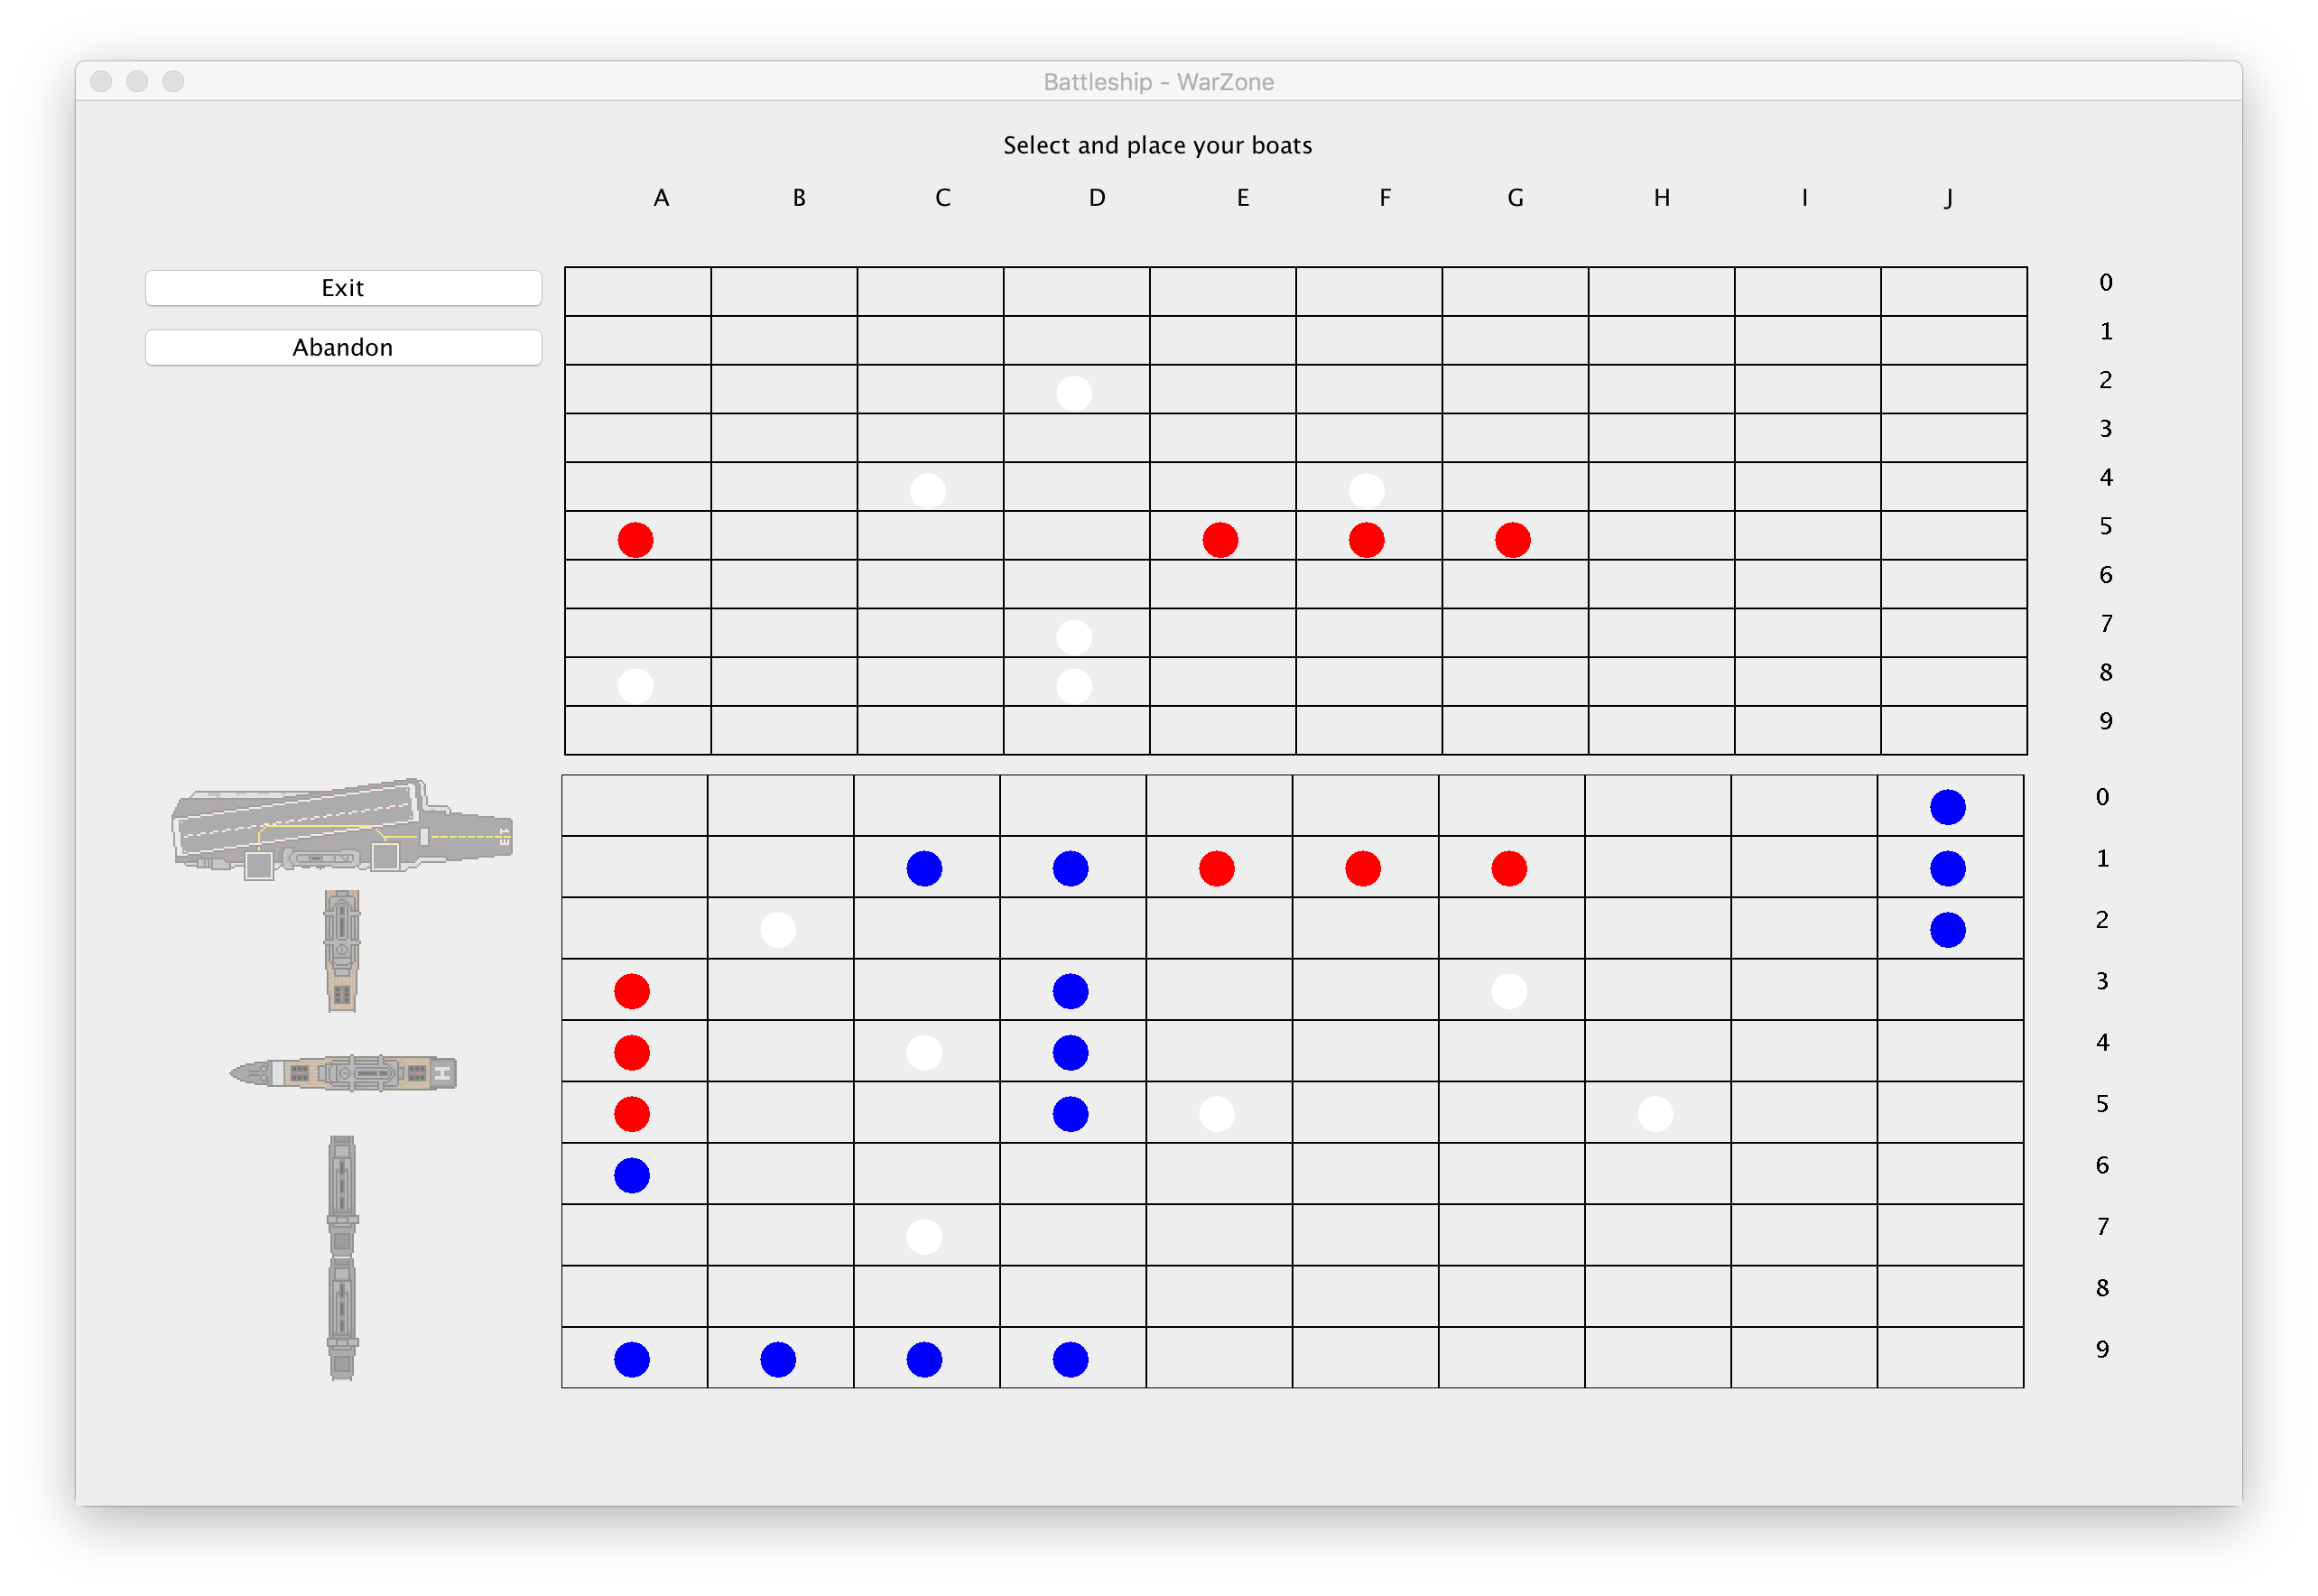
\includegraphics[scale=0.35]{images/touched}
    \caption{L'attaquant a touché un ou plusieurs bateaux}
    \label{fig:my_label}
\end{figure}

\begin{figure}[H]
    \center
    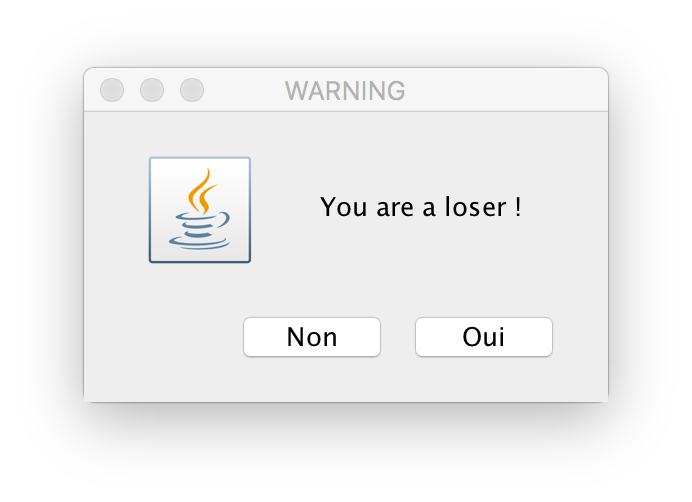
\includegraphics[scale=0.45]{images/loser}
    \caption{On est nul et on a perdu}
    \label{fig:my_label}
\end{figure}

\newpage

\end{document}